\chapter{Titre chapitre 1}
\lhead{\textit{Chapitre \thechapter: }}
\rhead{\textit{Titre chapitre \thechapter}}

\section{Introduction}
Insérez ici le texte d’introduction du chapitre et l’objectif à atteindre.



\section{Section 2}
Dans cette section....
\subsection{Sous section 1}

\subsection{Sous section 2}
\subsection{Exemple de tableau}
Le tableau \ref{tab:titretableau} suivant présente...
\begin{table}[h]
	\begin{center}
		\begin{tabular}{|l|l|}
			\hline
			\textbf{Température en C} & \textbf{Température en F} \\
			\hline
			\hline
			0 & ... \\
			\hline
			1 & ... \\
			\hline
			3 & ... \\
			\hline
			... & ... \\
			\hline
		\end{tabular}
	\end{center}
	\caption{Titre du tableau}
	\label{tab:titretableau}
\end{table}

\paragraph{}
L'informatique\footnote{Note bas de page "info.."} est...

\paragraph{}
Le système informatique...

\section{Section 3}
Dans cette section....
\section{Section 4}
Dans cette section....

\subsection{Exemple de figure}
\begin{figure}[h]
\centering
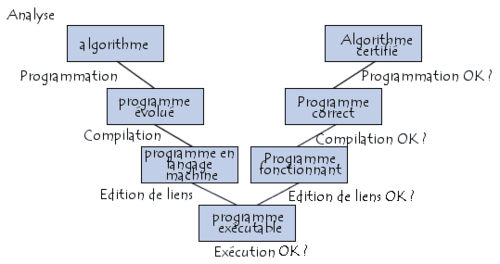
\includegraphics[width=15cm, height=6cm]{Imag/Fig1}
\caption{Titre de la figure}
\label{fig:Fig1}
\end{figure}
La figure \ref{fig:Fig1} présente...
\section{Section 4}
\section{Conclusion}
